% TELFOR 2026, IEEE conference paper (A4, two-column, four-page limit).
% Build (from paper/):  tectonic telfor_safe_selector.tex
%   (with TeX Live instead: pdflatex -> bibtex -> pdflatex x2.)
% Needs refs.bib and figures/budget_curve.pdf. The figure and every selector
% number are recomputed from frozen per-program records by
%   python3 scripts/verify_budgeted_selector.py
%   python3 scripts/generate_budget_figure.py
% The audit-framed alternative of the same material is telfor_revised.tex.
% The IEEE copyright notice is inserted by TELFOR for IEEE Xplore; keep the
% \IEEEpubid lines commented unless the camera-ready instructions say otherwise.

\documentclass[conference,a4paper]{IEEEtran}
\usepackage[utf8]{inputenc}
\usepackage[T1]{fontenc}
\usepackage{graphicx}
\usepackage{booktabs}
\usepackage{amsmath}
\setlength{\textfloatsep}{6pt plus 2pt minus 3pt}
\setlength{\dbltextfloatsep}{6pt plus 2pt minus 3pt}
\setlength{\floatsep}{6pt plus 2pt minus 2pt}
\setlength{\abovecaptionskip}{3pt}

% \IEEEoverridecommandlockouts
% \IEEEpubid{\makebox[\columnwidth]{XXX-X-XXXX-XXXX-X/26/\$31.00~\copyright2026 IEEE \hfill}}

\begin{document}

\title{Budgeted Code-Size Selection\\
with an LLVM \texttt{-Oz} Fallback}

\author{\IEEEauthorblockN{Dimitrije Pe\v{s}i\'c}
\IEEEauthorblockA{\textit{School of Electrical Engineering, University of Belgrade}\\
Belgrade, Serbia\\
pd230014d@student.etf.bg.ac.rs}}

\maketitle

\begin{abstract}
Choosing an LLVM pass sequence by IR instruction count can produce
larger machine code than the compiler's own size optimization. We
evaluate a budgeted selector: apply eight candidate sequences,
shortlist them by instruction count, measure native code bytes only
for the shortlist, and keep the \texttt{-Oz} object when it is smaller.
A retrospective study of frozen CompilerGym LLVM~10 records covers
347 programs, graph-neural and random candidate pools, and a reference
prepared with matching size attributes. Measuring two candidates plus
the reference saves 3.46--4.33\% of summed code-section bytes, falling
to 1.34--1.60\% without the dominant NPB suite. The fallback contributes
more than increasing the measurement budget, and prevents regressions
only in the protected metric. Instruction count helps shortlist
unordered candidates, while a fixed prefix is competitive for a mined
portfolio. No consistent byte-size advantage of learned generation is
observed. A causal audit explains how missing size attributes had
inflated the original comparison through reference-loop unrolling.
The study quantifies established selection mechanisms under a matched
reference; the retrospective measurement budget does not establish
an end-to-end speedup.
\end{abstract}

\begin{IEEEkeywords}
compiler optimization, LLVM, phase ordering, code size, reinforcement
learning, evaluation methodology
\end{IEEEkeywords}

\section{Introduction}
A compiler lowers a program to an intermediate representation (IR),
transforms it with a sequence of optimization passes, and only then
generates machine code. Work on learned pass ordering usually scores a
pass sequence by the number of IR instructions it leaves, the
\emph{instruction count} (IC), because IC is cheap and independent of
the target. IC is nevertheless a proxy. What is deployed is bytes of
machine code, and the code generator makes its own size decisions:
instruction selection, encodings, alignment padding and duplicated
loop tests change the byte count of unchanged IR. A lower IC therefore
does not guarantee smaller code, and a sequence chosen by IC can
produce a larger object than the compiler's own \texttt{-Oz}.

Choosing a pass order per program, the \emph{phase-ordering problem},
is undecidable in general~\cite{touati2006} and exhaustively searchable
only with heavy pruning~\cite{kulkarni2006}; searching pass orders
specifically for code size goes back at least to Cooper et
al.~\cite{cooper1999}. Reinforcement learning has since been used to
propose program-specific
orderings~\cite{autophase,compilergym,posetrl,coreset,mammadli};
CompilerGym~\cite{compilergym} standardized the environments and
exposes both IC and object-size observations, and its authors report
that plain random search is a competitive baseline. POSET-RL~\cite{posetrl}
chooses subsequences derived from \texttt{-Oz}, while the coreset
method~\cite{coreset} predicts a sequence from a small mined set.
MLGO~\cite{mlgo} trains an inlining policy directly
against native size, and ProGraML~\cite{programl} motivated the graph
representation used by our policy.

This paper asks a practical question about such searches: given a
handful of candidate sequences, however produced, how should the final
object be chosen so that the result is useful and never worse than
\texttt{-Oz}, and how much native measurement does that require? We
answer it on an existing experiment, a graph-neural-network (GNN)
policy, a mined sequence portfolio and random search in CompilerGym,
without retraining. The contributions are: (1)~a \emph{baseline-safe
budgeted selector} and its budget--quality curve for one to eight native
measurements, with a decomposition into the contributions of the
fallback, the byte measurement and the IC shortlist; (2)~a control that
quantifies what IC is worth as a shortlist against measuring the same
number of arbitrary candidates; (3)~a service-faithful causal audit of
the \texttt{-Oz} reference, which shows that a reference without size
attributes had inflated the experiment's earlier headline; and (4)~a
source-build control against a true \texttt{clang -Oz}. None of the
ingredients is new: a fallback, selection by measured bytes and fixed
portfolios are established tools. The contribution is their controlled,
reproducible quantification under a matched reference.

\section{Selector and Protocol}
\textbf{Selector.} Let a generator propose $n$ pass sequences for a
module; here $n{=}8$. The selector (i)~applies each sequence and reads
the IC of the result, (ii)~keeps the $k$ candidates with the lowest IC,
the first winning ties, (iii)~generates native code for these $k$
candidates and for the \texttt{-Oz} reference and measures their
code-section bytes, and (iv)~delivers the smallest object, a tie going
to \texttt{-Oz}. The delivered object is never larger than the
\texttt{-Oz} object in the measured metric. That property follows from
the rule and is not an empirical finding; it says nothing about other
metrics or about semantics. The cost is $n$ sequence applications plus
$k{+}1$ code generations. With $k{=}n$ the rule is full byte selection;
with $k{=}1$ it is the conventional IC rule plus the fallback. A
stricter variant accepts a candidate only if it is no larger than
\texttt{-Oz} in \emph{both} object metrics defined below.

\textbf{Environment and reference.} All records come from the unmodified
CompilerGym~0.2.5 service with its bundled LLVM~10. The reference is the
service's own \texttt{-Oz} baseline path; command-line \texttt{opt -Oz}
builds a different pipeline and is never used. The environment's modules
carry no size attributes, whereas \texttt{clang -Oz} attaches
\texttt{minsize} and \texttt{optsize} to every function definition. We
therefore add both attributes to every definition, keeping the target
triple and data layout, and give the \emph{same} prepared module to the
reference and to every candidate. Section~\ref{sec:causal} shows what
happens otherwise.

\textbf{Cohorts and generators.} Three cohorts are kept apart. The
\emph{portfolio cohort} has 210 modules (120 NPB, 40
MiBench~\cite{mibench}, 50 BLAS) with two pools of eight sequences: a
portfolio mined on separate training programs before this study, and
random search. The \emph{selector cohort} has 347 programs (the same
210 plus 12 CHStone~\cite{chstone}, 28 csmith~\cite{csmith} and 97
POJ-104) with eight pools: three checkpoints of a GNN policy from our
earlier experiment (training seeds 42, 123, 456), each contributing the
eight episodes it sampled on the prepared input, and five realizations
of eight uniformly random sequences. Every sequence has 45 actions from
the same 36-pass space; pools are never merged. The \emph{source
control} has the 12 CHStone programs compiled from C.

\textbf{Metrics.} We record IC and two sizes of the relocatable x86-64
object emitted by the bundled \texttt{llc}: \emph{code-section bytes},
the sum of the \texttt{.text} sections, and \emph{Berkeley text}, the
\texttt{text} column of \texttt{llvm-size}, which also counts other
read-only allocated sections such as constants and unwind tables.
Neither is the footprint of a linked binary. A saving is
$100\,(\sum \text{ref} - \sum \text{sel})/\sum \text{ref}$ over the
stated cohort, a ratio of sums that weights large modules more. Ranges
are minima and maxima over checkpoints or realizations, not confidence
intervals.

\textbf{Retrospective evaluation.} The frozen campaigns measured all
eight candidates of every pool and program. Every rule is therefore
recomputed exactly from the records, with no new compiler run for the
selector analysis; the budget curve is a counterfactual over measured candidates,
not a timed end-to-end run. As a control for the IC shortlist we compute
the exact mean saving when $k$ \emph{arbitrary} candidates of the same
pool are measured, over all $\binom{8}{k}$ subsets, with the same
fallback. This is a plain byte-driven search with a budget of $k$
sequences.

\begin{figure*}[t]
\centering
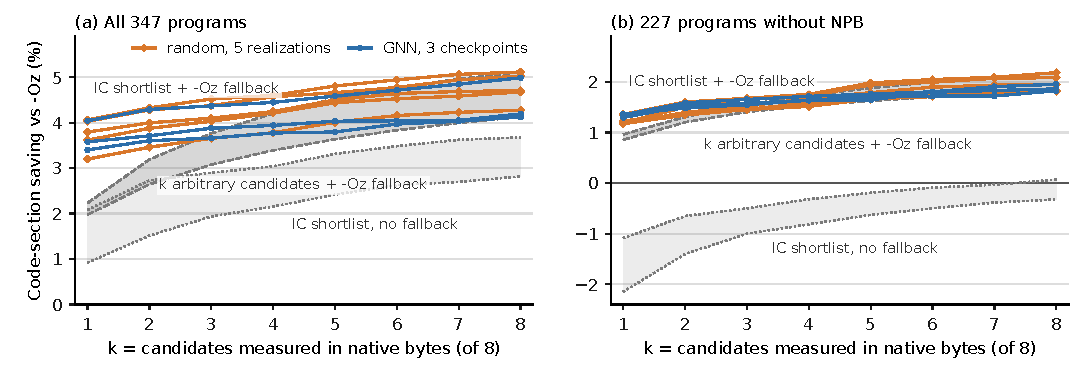
\includegraphics[width=\textwidth]{figures/budget_curve.pdf}
\caption{Budget--quality curves of the baseline-safe selector on the
selector cohort; reference: service \texttt{-Oz} with size attributes.
Lines: IC shortlist of $k$ candidates, byte selection, \texttt{-Oz}
fallback, one line per GNN checkpoint or random realization. Dashed
band: $k$ arbitrary candidates with the same fallback (exact mean over
all subsets; minimum and maximum over the eight pools). Dotted band: the
same IC shortlist without the fallback. At $k{=}8$ the shortlist and the
arbitrary choice coincide. Retrospective recomputation from measured
candidates.}
\label{fig:budget}
\end{figure*}

\section{Results}

\subsection{Portfolio cohort: fallback and measurement budget}
Table~\ref{tab:headline} gives the portfolio cohort. The conventional
rule, the lowest-IC candidate with no fallback, saves 3.48\%
(portfolio) and 3.89\% (random) of code-section bytes over 210 modules.
Keeping \texttt{-Oz} when it is smaller raises this to 4.17\% and
4.62\% with a single native measurement per program besides the
reference, and measuring all eight candidates gives 4.90\% and 5.88\%.
The saving is positive in each suite, from 2.47\% on BLAS to 8.80\% on
NPB. Random search is at least as good as the mined portfolio in the
pooled rows at every budget, so the pool's origin is not what produces
the saving. For an ordered portfolio a fixed prefix is a natural
alternative shortlist: measuring only its first two or three sequences,
with the fallback, saves 4.42\% and 4.62\% while applying two or three
sequences instead of eight, more than the IC shortlist of the same size
(4.35\%, 4.40\%). For the portfolio the IC shortlist is clearly ahead
only at $k{=}1$ (4.17\% against 2.74\% for the first sequence alone).

\begin{table}[t]
\caption{Portfolio cohort: code-section saving (\%) over the attributed
service \texttt{-Oz}. IC: lowest-IC candidate, no fallback. S$k$: IC
shortlist of $k$, byte selection, \texttt{-Oz} fallback; S8 measures
all eight.}
\label{tab:headline}
\centering
\footnotesize
\setlength{\tabcolsep}{3.6pt}
\begin{tabular}{llrrrrr}
\toprule
Suite ($n$) & Pool & IC & S1 & S2 & S4 & S8 \\
\midrule
NPB (120)    & portfolio & 5.76 & 6.36 & 6.53 & 6.70 & 7.09 \\
             & random    & 6.46 & 7.35 & 7.63 & 8.28 & 8.80 \\
MiBench (40) & portfolio & 1.47 & 2.72 & 2.81 & 2.86 & 3.13 \\
             & random    & 1.00 & 2.11 & 2.21 & 2.41 & 4.35 \\
BLAS (50)    & portfolio & 0.95 & 1.69 & 1.88 & 2.13 & 2.47 \\
             & random    & 1.14 & 1.62 & 1.93 & 2.14 & 2.50 \\
\midrule
All (210)    & portfolio & 3.48 & 4.17 & 4.35 & 4.54 & \textbf{4.90} \\
             & random    & 3.89 & 4.62 & 4.90 & 5.34 & \textbf{5.88} \\
\bottomrule
\end{tabular}
\end{table}

\subsection{Budget curve and the three contributions}
Fig.~\ref{fig:budget}(a) shows the selector cohort of 347 programs. The
three contributions separate cleanly. \emph{Fallback:} the conventional
IC rule saves 1.55--2.08\% for the three GNN checkpoints and
0.92--2.05\% for the five random realizations; adding only the fallback
($k{=}1$) gives 3.40--4.04\% and 3.20--4.06\%. This is the largest single
step. \emph{Budget:} measuring two candidates gives 3.60--4.29\% (GNN)
and 3.46--4.33\% (random), four give 3.77--4.45\% and 3.78--4.60\%, and
all eight give 4.13--4.99\% and 4.27--5.11\%. \emph{Shortlist:} at equal
$k$ the IC shortlist beats $k$ arbitrary candidates by 1.15--1.93
percentage points at $k{=}1$, by 0.60--1.22 at $k{=}2$ and by 0.15--0.45 at
$k{=}4$, across the eight pools; a plain byte search needs three to five
measured candidates to match the IC shortlist of one. IC is thus a poor
final selector and a useful shortlist.

\emph{Generator:} the GNN and random lines interleave at every $k$. The
GNN keeps a lower summed IC than every random realization under the IC
rule, so the policy is better at the objective it was trained on, but
in delivered bytes we find no consistent advantage for either
generator. This is not a demonstration of equivalence: no equivalence
test was run and resampling a checkpoint was not measured.

\subsection{Without NPB, and per suite}
NPB carries most of the pooled saving, so Fig.~\ref{fig:budget}(b)
repeats the analysis on the 227 other programs. Without the fallback
the aggregate is close to zero or negative, from $-2.15\%$ to $-1.09\%$ at
$k{=}1$ and from $-0.32\%$ to $+0.07\%$ at $k{=}8$: gains on some suites are
cancelled by regressions on others. With the fallback the saving is
1.17--1.36\% at $k{=}1$, 1.34--1.60\% at $k{=}2$ and 1.81--2.18\% at
$k{=}8$ over the eight pools. The shortlist advantage is smaller here, at
most 0.46 points at $k{=}1$ and at most 0.10 by $k{=}4$. Per suite at $k{=}8$
the eight pools save 7.87--10.33\% on NPB, 2.86--4.35\% on MiBench,
2.75--4.18\% on POJ-104, 2.19--2.50\% on BLAS, 1.05--1.59\% on CHStone and
0.04--0.84\% on csmith, where \texttt{-Oz} is almost always kept. The
saving is not spread evenly over programs either: at $k{=}2$ the selector
improves 163--177 of the 347 programs and returns \texttt{-Oz} for the
rest, and at $k{=}8$ it improves 198--205; the median saving among improved
programs is 3.1--3.6\%.

\subsection{What the fallback protects}
The guarantee covers the metric that is selected on and no other. With
the code-section fallback at $k{=}8$, the delivered objects are smaller
than \texttt{-Oz} in summed Berkeley text as well, by 1.74--2.82\%, yet
45--64 of the 347 programs receive an object with a \emph{larger}
Berkeley text than \texttt{-Oz}. The stricter variant, which accepts a
candidate only if neither metric grows, removes all such cases; it
saves 3.75--4.88\% of code-section bytes instead of 4.13--5.11\% and
2.39--3.30\% of Berkeley text. Both sizes are read from the same object,
so the stricter rule needs no further measurement. Which metric should
be protected depends on the deployment target, and neither is a linked
footprint.

\subsection{Cost}
We did not time the selector end to end. In the frozen campaign, which
ran in an emulated amd64 container, applying one 45-action sequence in
the service took 13.7\,ms on average and one object measurement, which
spawns the code generator and size tools as processes, 451\,ms.
These include audit overhead; the native ratio is unknown. Excluding
generator inference and common reference preparation, a constant-cost
model gives $8s+2m$ for sequence cost $s$ and
measurement cost $m$, and the plain search that matches it with $j$
candidates costs $js+(j{+}1)m$; the shortlist is cheaper whenever
$m/s>(8{-}j)/(j{-}1)$, that is, above 2.5 for $j{=}3$ and above 0.75 for
$j{=}5$.

\section{Why the Reference Must Be Prepared}
\label{sec:causal}
\begin{table}[t]
\caption{Service \texttt{-Oz} reference on 120 NPB modules (sums).
P: plain input; U: plain input, unrolling disabled; A: size
attributes.}
\label{tab:causal}
\centering
\footnotesize
\setlength{\tabcolsep}{3.5pt}
\begin{tabular}{lrrrrr}
\toprule
Metric & P & U & A & P$-$U & P$-$A \\
\midrule
IR instructions    & 53,085  & 40,525  & 40,446  & 12,560 & 12,639 \\
Code-section bytes & 291,616 & 234,913 & 214,296 & 56,703 & 77,320 \\
Berkeley text      & 348,878 & 290,559 & 267,814 & 58,319 & 81,064 \\
\bottomrule
\end{tabular}
\end{table}

The same experiment, evaluated by IC against the environment's plain
\texttt{-Oz} reference, had reported a large gain. On the 120 NPB
modules the mined portfolio's IC gain is 23.84\% with plain input (P)
and 0.08\% once reference and candidates carry the size attributes (A);
its code-section gain falls from 23.71\% to 5.76\%. A service-faithful
intervention identifies the cause. The service has no unrolling switch,
so we add \texttt{llvm.loop.unroll.disable} to every natural loop of
the plain input and run the unchanged service (U). With plain input the
\texttt{-Oz} pipeline fully unrolls constant-trip-count loops: LLVM
reports 449 unrolling remarks on 43 of the 120 modules, and none with
the attributes. A small replica of the service's pass-manager
construction, whose output IR equals the service's on every audited
input, is used only to read these remarks. Table~\ref{tab:causal} shows
that disabling unrolling alone removes 12,560 of the 12,639 IC by which
P exceeds A; on each of the 43 modules U has exactly the IC of A. The
residual 79 IC lies on five modules without unrolling, where IR diffs
point to attribute-sensitive inlining and instruction combining, which
we did not ablate.

Bytes behave differently: unrolling accounts for 56,703 of the 77,320
code-section bytes between P and A. For the remaining 20,617 bytes a
fixed-IR control, which adds the attributes to U's optimized output so
that only code generation sees them, saves 20,402 bytes and leaves U
215 bytes above A. We therefore do not call the 20,617 bytes purely a
code-generation effect, and since the byte effect of the attributes
depends on whether unrolling has already happened, we report
differences of sums rather than shares. One function makes the
mechanism concrete (Table~\ref{tab:small}a): \texttt{transfb\_nc0} of
NPB-116 holds a $5{\times}3$ loop nest that the plain reference expands
into 15 body copies, more IR instructions than the unoptimized input
has; with unrolling disabled the loop survives, and code generation
under the attributes alone then shrinks it further. The function was
extracted unchanged with LLVM's own tool; no corresponding C source was
used or reconstructed. The causal result is established for NPB only.



\begin{table}[t]
\caption{(a) Causal example, function \texttt{transfb\_nc0} of NPB-116.
(b) Source-build control on 12 CHStone programs.}
\label{tab:small}
\centering
\footnotesize
\setlength{\tabcolsep}{4pt}
\begin{tabular}{lrrr}
\toprule
(a) One function & P & U & A \\
\midrule
IR instructions & 90 & 25 & 25 \\
Function bytes  & 377 & 119 & 87 \\
\midrule
(b) 12 programs & \texttt{clang -Oz} & Selected & Saving \\
\midrule
Code-section bytes & 32,123 & 31,729 & 1.23\% \\
Improved / reference kept & \multicolumn{3}{r}{5 / 7} \\
\bottomrule
\end{tabular}
\end{table}

\textbf{Source-build control.} The attributed service reference is
still not a source build. We therefore compiled the 12 CHStone programs
from C with \texttt{clang -Oz} and ran the selector with that object as
the fallback and the first three portfolio sequences as candidates
(Table~\ref{tab:small}b). Summed code sections fall from 32,123 to
31,729 bytes, a saving of 1.23\%; five programs improve and seven keep
the \texttt{clang -Oz} object. All evaluated objects pass the
benchmarks' fixed-vector tests, which is a regression check and not a
proof of semantic equivalence. The saving is comparable in size to the
CHStone result of the selector cohort above, which uses the service
reference. Measuring the saved linked executables, with hashes matched
to the recorded tests, retains the 394-byte code saving (1.13\% of linked
\texttt{.text}). Summed Berkeley text falls by only 0.15\%, with one
program regressing; total ELF file bytes fall by 0.05\%. These are
unstripped, dynamically linked executables built with \texttt{-no-pie},
excluding shared-library contents. Object-code protection therefore
does not imply a footprint guarantee.

\section{Limitations}
All results concern one software stack, CompilerGym 0.2.5 with LLVM~10
and x86-64 objects, one 36-pass action space and the stated cohorts.
The budget curve is retrospective and its budgets were not fixed in
advance, which is why the whole curve is shown; no end-to-end time or
runtime of the generated code was measured. Savings are ratios of sums
dominated by NPB, and 41--53\% of the programs, depending on the
budget, gain nothing. Modules
of a suite are related, so 43 unrolled NPB modules are not 43
independent confirmations, and three checkpoints with five realizations
are not fifteen independent experiments. Stored instruction counts
reproduce exactly, but bit-identical outputs are not guaranteed: one
never-selected csmith candidate has two object hashes with identical
metrics. Except for the small CHStone control, sizes are relocatable objects.
Fixed-vector tests
are not semantic proofs.

\section{Conclusion}
A pass-ordering search can avoid growth in a chosen object-size metric:
prepare the reference and the candidates with
the attributes of a real size build, measure native bytes for a short
IC-ranked list, and keep \texttt{-Oz} when it is smaller. In this
experiment, measuring two candidates plus the reference saves
3.46--4.33\% of code-section bytes on 347 programs, and 1.34--1.60\%
without NPB. The source-build control saves 1.23\% in object code but
only 0.05\% in total linked-file bytes. The fallback prevents growth in
the protected metric, while learned candidate generation shows no
consistent byte-size advantage. The fallback and the reference
preparation matter most, the IC shortlist is worth two to four native
measurements on the full cohort and less without NPB, and the
generator matters least. Evaluations of learned
phase ordering for size should report a matched reference, the
selection metric, a random-search control and the fallback result
alongside the raw one.

\textbf{Reproducibility.} Frozen protocols, per-program records,
independent verification reports and the scripts that recompute every
number and the figure are in the \texttt{results} and \texttt{scripts}
directories of the project repository;\footnote{\raggedright
\texttt{https://github.com/dimitrijepesic/compiler-opt}} a claim audit
in the \texttt{paper} directory maps each number to its record.

\section*{Acknowledgment}
The author thanks Prof.~Zaharije Radivojevi\'c for early discussions of this
work.

\bibliographystyle{IEEEtran}
\bibliography{refs}

\end{document}
